\section{Desarrollo de Benchmarks}

El establecimiento de marcos de evaluación estandarizados ha sido crucial para avanzar en la investigación de la detección de anomalías. El Numenta Anomaly Benchmark (\textbf{NAB}), introducido en 2015, proporcionó el primer entorno controlado y repetible para probar algoritmos de detección de anomalías en tiempo real sobre datos de transmisión \cite{lavin_evaluating_2015}. NAB abordó la necesidad crítica de puntos de referencia que pudieran evaluar detectores que procesan datos en tiempo real en lugar de lotes, con algoritmos de puntuación diseñados específicamente para las características de los datos de transmisión.

Sin embargo, investigaciones posteriores han revelado limitaciones significativas en los conjuntos de datos de evaluación más populares. Un análisis crítico publicado en 2020 demostró que la mayoría de los ejemplares individuales en conjuntos de datos ampliamente utilizados sufren de cuatro fallas fundamentales, lo que sugiere que muchas comparaciones de algoritmos publicadas pueden ser poco confiables y que el progreso aparente en los últimos años puede ser ilusorio. Este análisis llevó a la introducción del \textbf{UCR Time Series Anomaly Archive} en el año 2020, que tiene como objetivo proporcionar comparaciones significativas entre enfoques y una medición precisa del progreso \cite{wu_current_2023}.

En la Figura \ref{fig:Evolución de la detección de anomalía} se visualiza dicha evolución de detección de anomalías. Donde el eje y representa las categorías y en el eje x los años donde se comenzó a poner en práctica dicho método en la detección de anomalía en series temporales.


\begin{figure}
    \centering
    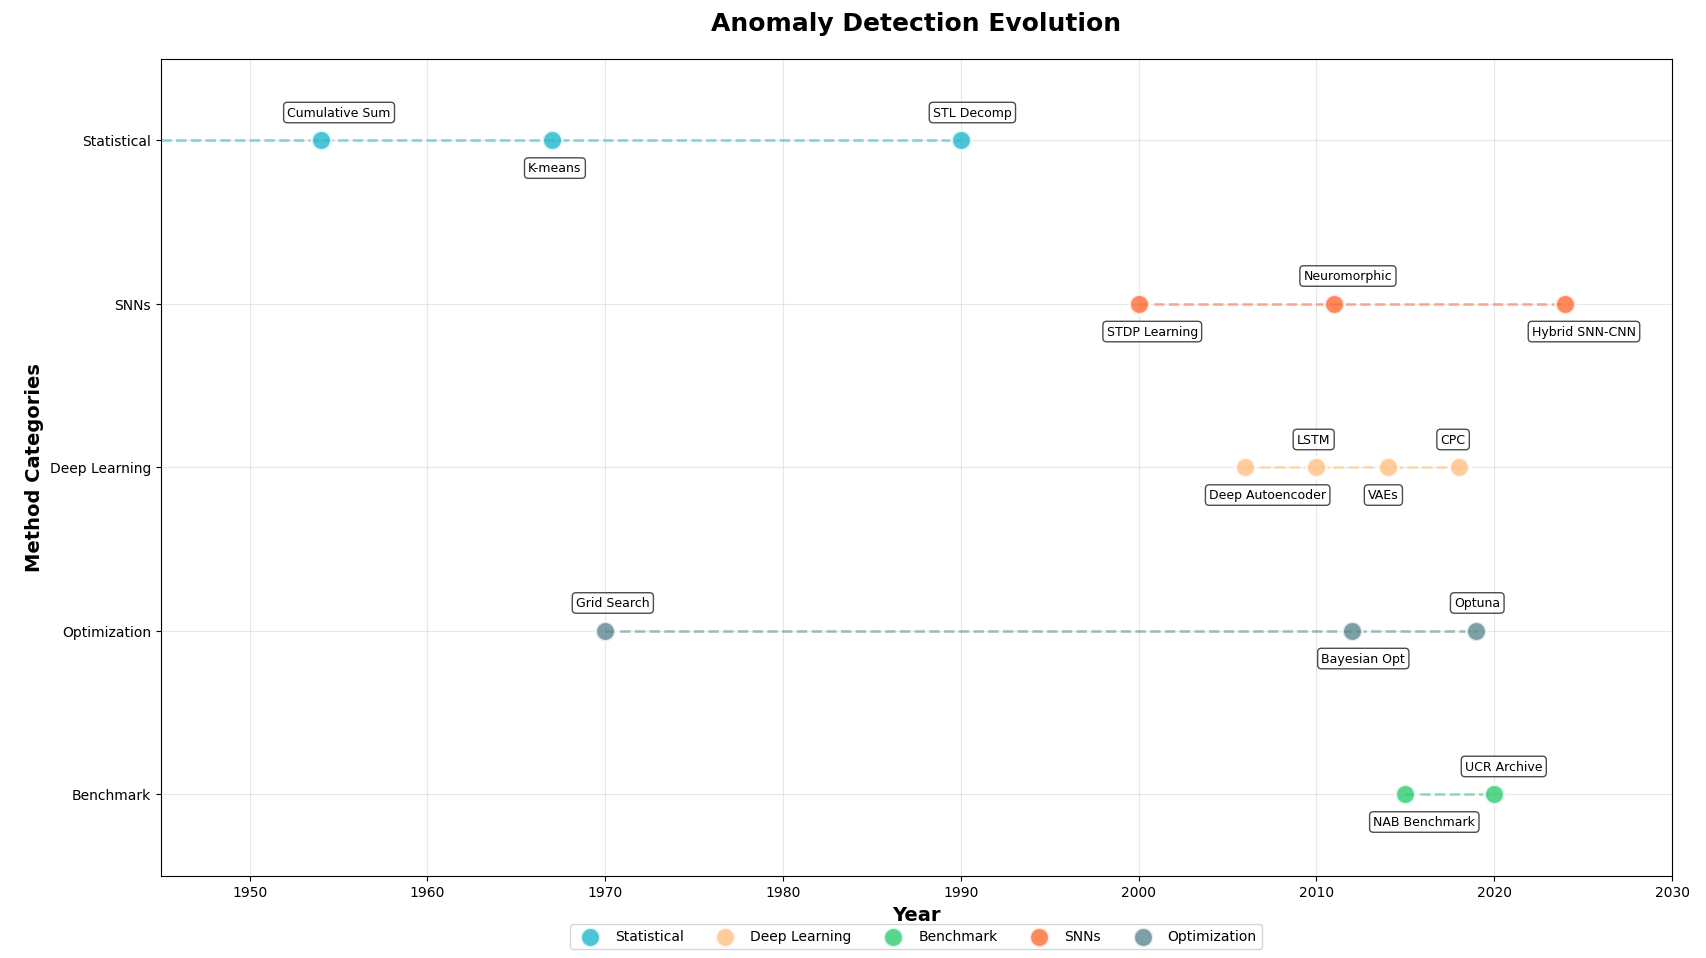
\includegraphics[width=\paperwidth,height=\paperheight,keepaspectratio,angle=90]{Imagenes/Anomaly Detection Evolution.png}
    \caption{Evolución de la detección de anomalía. Fuente: Elaboración propia.}
    \label{fig:Evolución de la detección de anomalía}
\end{figure}